\documentclass[10pt]{beamer}

\usepackage{appendixnumberbeamer}

% \usepackage{beamerposter}

\usepackage{fontspec}
\usepackage{csquotes}
\usepackage[main=english]{babel}
\babelprovide[import, onchar=ids fonts letters]{ancientgreek}

\usepackage{linguex}
\usepackage{tikz} %for all basic options
\usepackage{tikz-qtree} %for simple tree syntax
\usepackage{booktabs}
\usepackage[normalem]{ulem}
\usepackage{hyphenat}
\usepackage{multirow}
\usepackage{pgfplots}
\usepackage{paralist}
\usepackage[
  backend=biber,
  uniquename=init,
  giveninits,
  dashed=true,
  style=authoryear-comp
  ]{biblatex}
\addbibresource{./biblio.bib}

\usetheme[
	progressbar=foot,
	sectionpage=progressbar,
	numbering=fraction]{metropolis}

\newcommand\Wider[2][4em]{%
	\makebox[\linewidth][c]{%
		\begin{minipage}{\dimexpr\textwidth+#1\relax}
			\raggedright#2
		\end{minipage}%
	}%
}

\title{Rethinking case attraction on Ancient Greek infinitive clauses}
\author{Caio B. A. Geraldes\newline<\texttt{caio.geraldes@usp.br}>\vspace{5pt}}
\date{June 25, 2025}
\institute{Universidade de São Paulo\\
\includegraphics[height=0.40cm]{logo-fapesp.png}}

\setsansfont{Fira Sans}
\setmonofont[Scale=0.75]{Noto Sans Mono}

\usepackage[
	backend=biber,
	style=authoryear,
	autolang=hyphen,
]{biblatex}
\addbibresource{biblio.bib}

\definecolor{obl}{RGB}{41,5,195}
\definecolor{teste}{RGB}{46,139,87}
\definecolor{verb}{RGB}{255, 0, 0}
\definecolor{acc}{RGB}{11,92,16}
\definecolor{atr}{RGB}{128,0,128}
\newcommand{\Vum}[1]{#1}
\newcommand{\Vdois}[1]{#1}
\newcommand{\Obl}[1]{\textcolor{obl}{\uline{#1}}}
\newcommand{\XAcu}[1]{\textcolor{acc}{\uline{#1}}}
\newcommand{\XObl}[1]{\textcolor{atr}{\uline{#1}}}
\newcommand{\vum}[1]{\textbf{#1}}
\newcommand{\vdois}[1]{\textbf{#1}}
\newcommand{\oobl}[1]{\textbf{#1}}
\newcommand{\xobl}[1]{\textbf{#1}}

\begin{document}

\maketitle

\begin{frame}
	\frametitle{Example}

	\ex.
	\a.συμβουλεύει \textbf{τῷ Ξενοφῶντι ἐλθόντα} {εἰς Δελφοὺς}
	ἀνακοινῶσαι {τῷ θεῷ} {περὶ τῆς πορείας}.\\
	He advices Xenophon to go to Delphi and ask the god about the travel.
	(Xen.\ \emph{Anab.} 3.1.5)
	\b.ἀφῆκε \textbf{μοι ἐλθόντι} {πρὸς ὑμᾶς} λέγειν τἀληθῆ.\\
	He allowed me to go and speak the truth in front of you.
	(Xen.\ \emph{Hell.} 6.1.13)


\end{frame}

\begin{frame}
	\frametitle{Direct Acyclic Graph: Agreement}
	Framework: \textcite{Corbett2006}

	Features of the \textbf{C}ontroller, \textbf{T}arget and \textbf{D}omain
	``cause'' non\hyp{}canonical \textbf{A}greement

	\begin{center}
		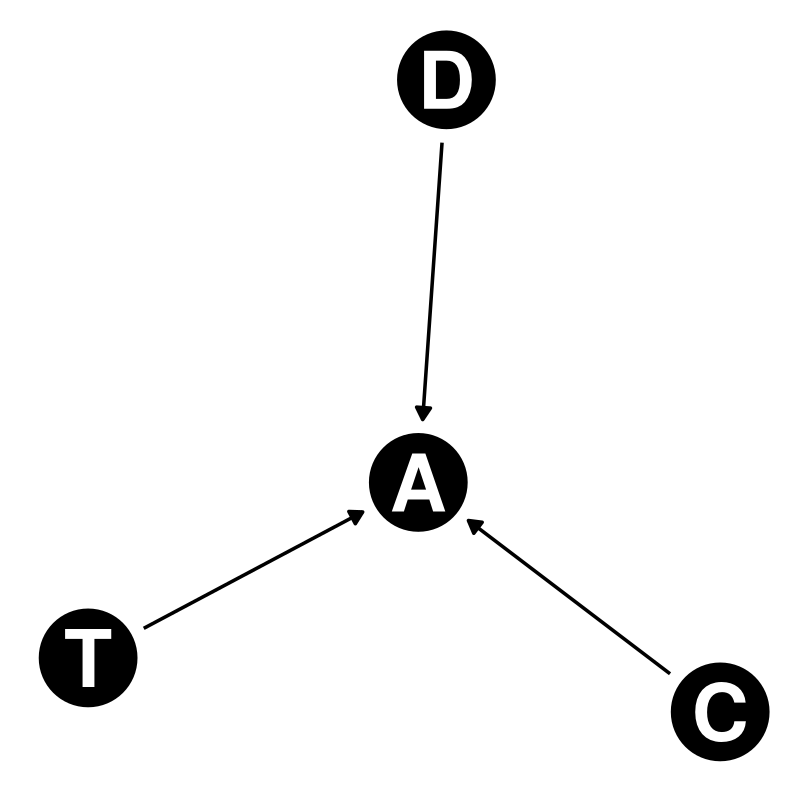
\includegraphics[width=0.40\textwidth]{../analysis/figs/dag_non_canonical_agreement.png}
	\end{center}
\end{frame}

\begin{frame}
	\frametitle{Domain of attraction:	Part of speech and copular infinitive}

	\ex. Agreement and Predicate Hierarchies~(\cite[233]{Corbett2006}):\\
	{\small
	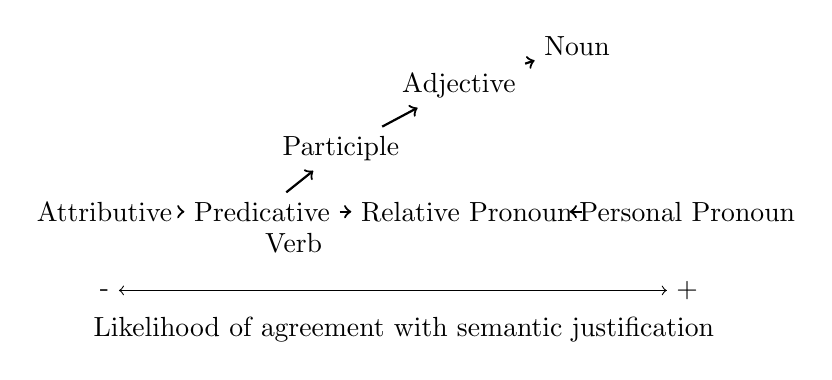
\begin{tikzpicture}[baseline=0pt]
    \node (attr) at (0, 0) {Attributive};
    \node (pred) at (2, 0) {Predicative};
    \node (predv) at (2.4, -0.4) {Verb};
    \node (predp) at (3.0, .8) {Participle};
    \node (preda) at (4.5, 1.6) {Adjective};
    \node (predn) at (6.0, 2.1) {Noun};
    \node (relp) at (4.6, 0) {Relative Pronoun};
    \node (perp) at (7.4, 0) {Personal Pronoun};
    \node (less) at (0, -1) {-};
    \node (plus) at (7.4, -1) {+};
    \draw[->, thick] (attr) to (pred);
    \draw[->, thick] (pred) to (relp);
    \draw[->, thick] (relp) to (perp);
    \draw[->, thick] (pred) to (predp);
    \draw[->, thick] (predp) to (preda);
    \draw[->, thick] (preda) to (predn);
    \draw[->] (less) to (plus);
    \draw[->] (plus) to (less);
    \node at (3.8, -1.5) {Likelihood of agreement with semantic justification};
\end{tikzpicture}
}

\end{frame}

\begin{frame}
	\frametitle{The domain of attraction: DAG}
	\begin{center}
	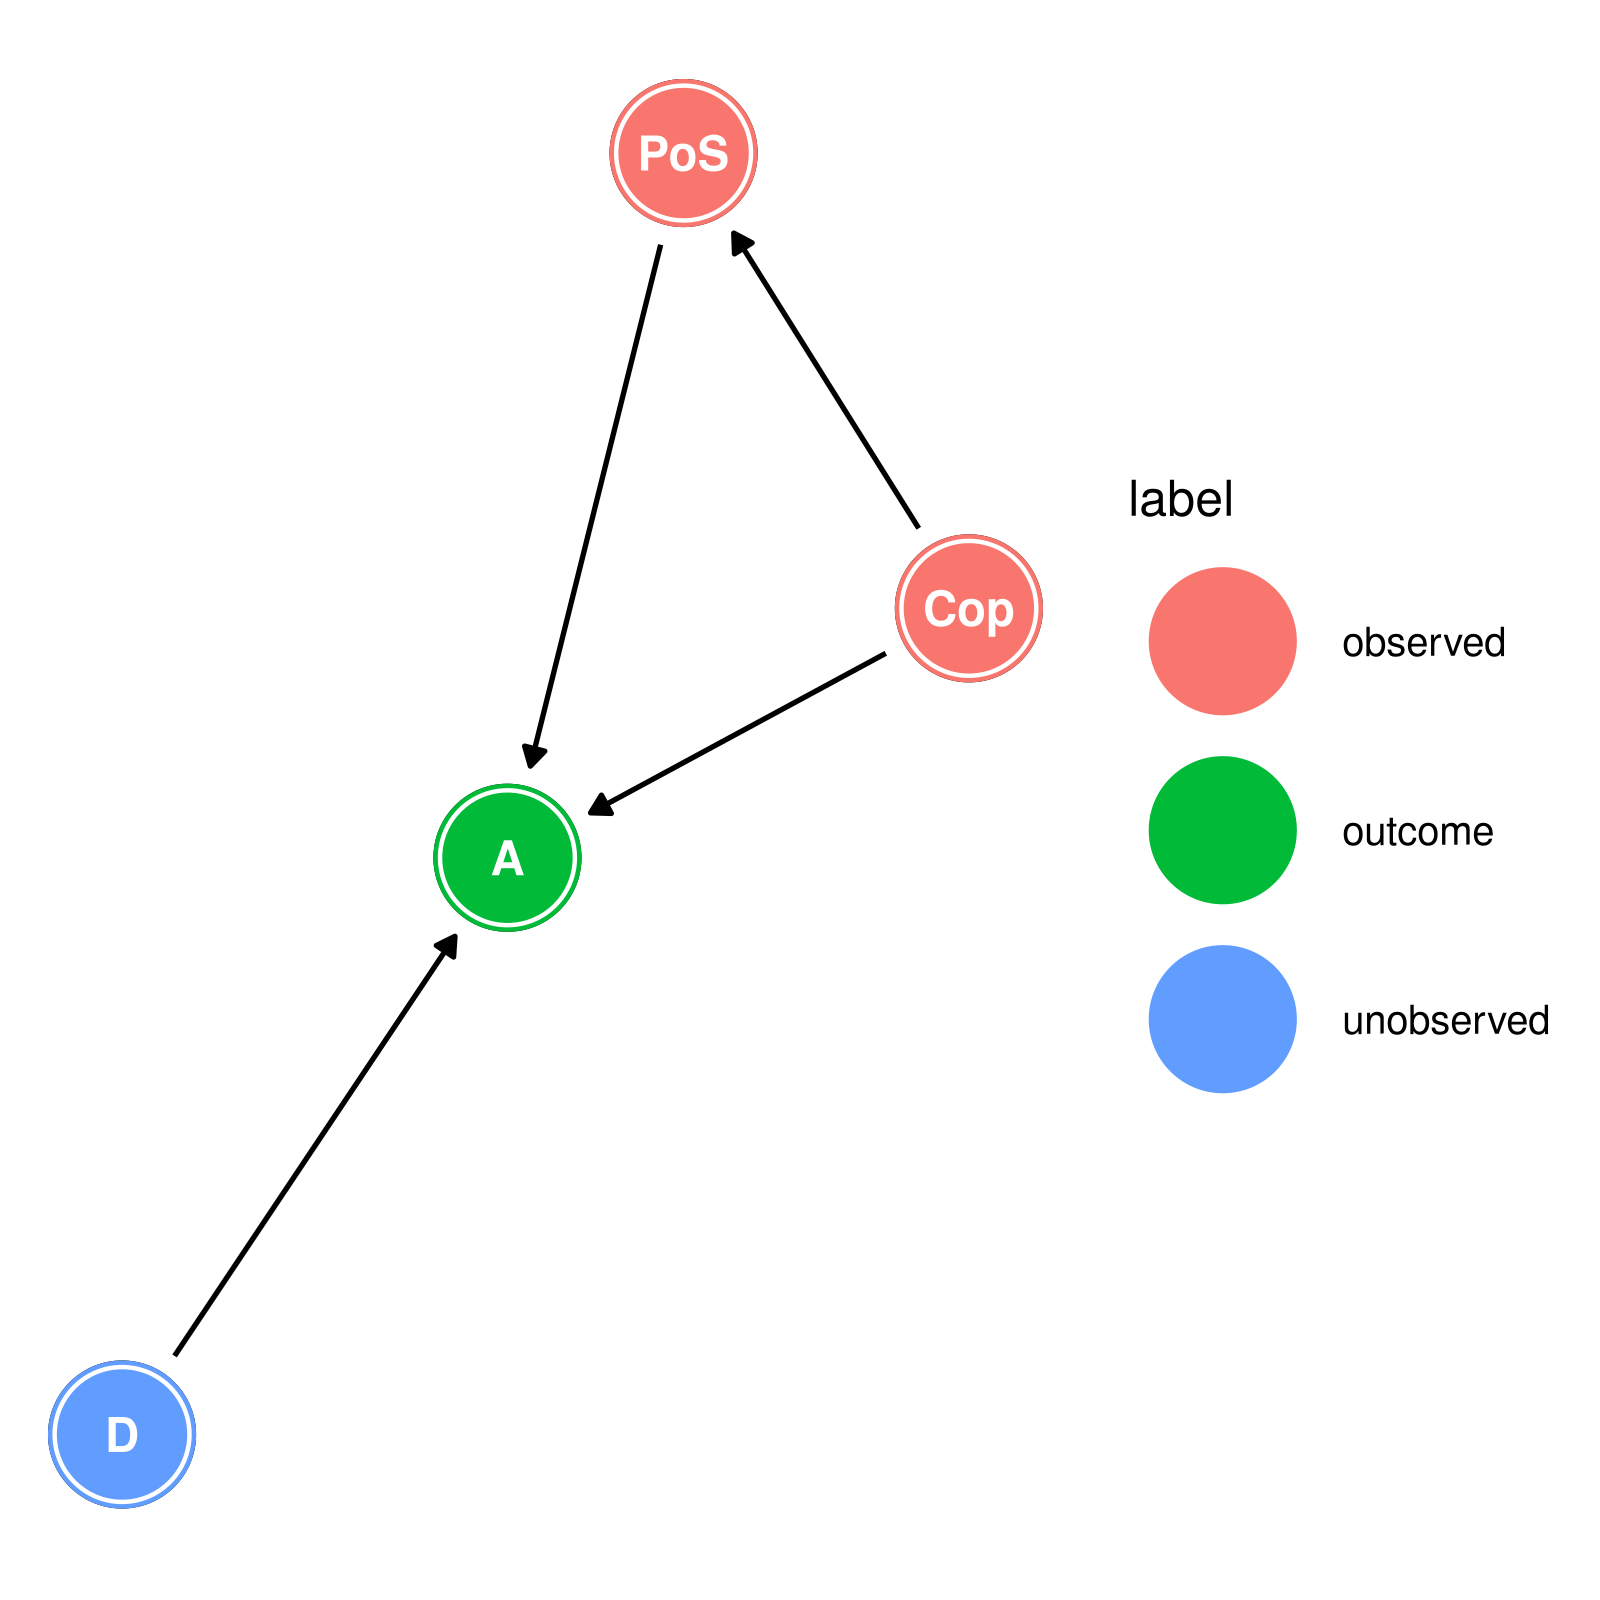
\includegraphics[width=0.65\linewidth]{../analysis/figs/dag_a.png}
	\end{center}
\end{frame}

\begin{frame}
\frametitle{The controller of attraction: Thematic role}
	\ex. ἀλλ᾽ ἐξαρκῇ \textbf{σοι} τὰ ἔργα αὐτῶν \textbf{ὁρῶντι} σέβεσθαι καὶ τιμᾶν
	τοὺς θεούς.\\
	But it is enough for you to look at these deeds and respect the gods. 
	(Xen.\ \emph{Mem.} 4.3.13)

\end{frame}

\begin{frame}
	\frametitle{The controller of attraction: DAG}
	\begin{center}
	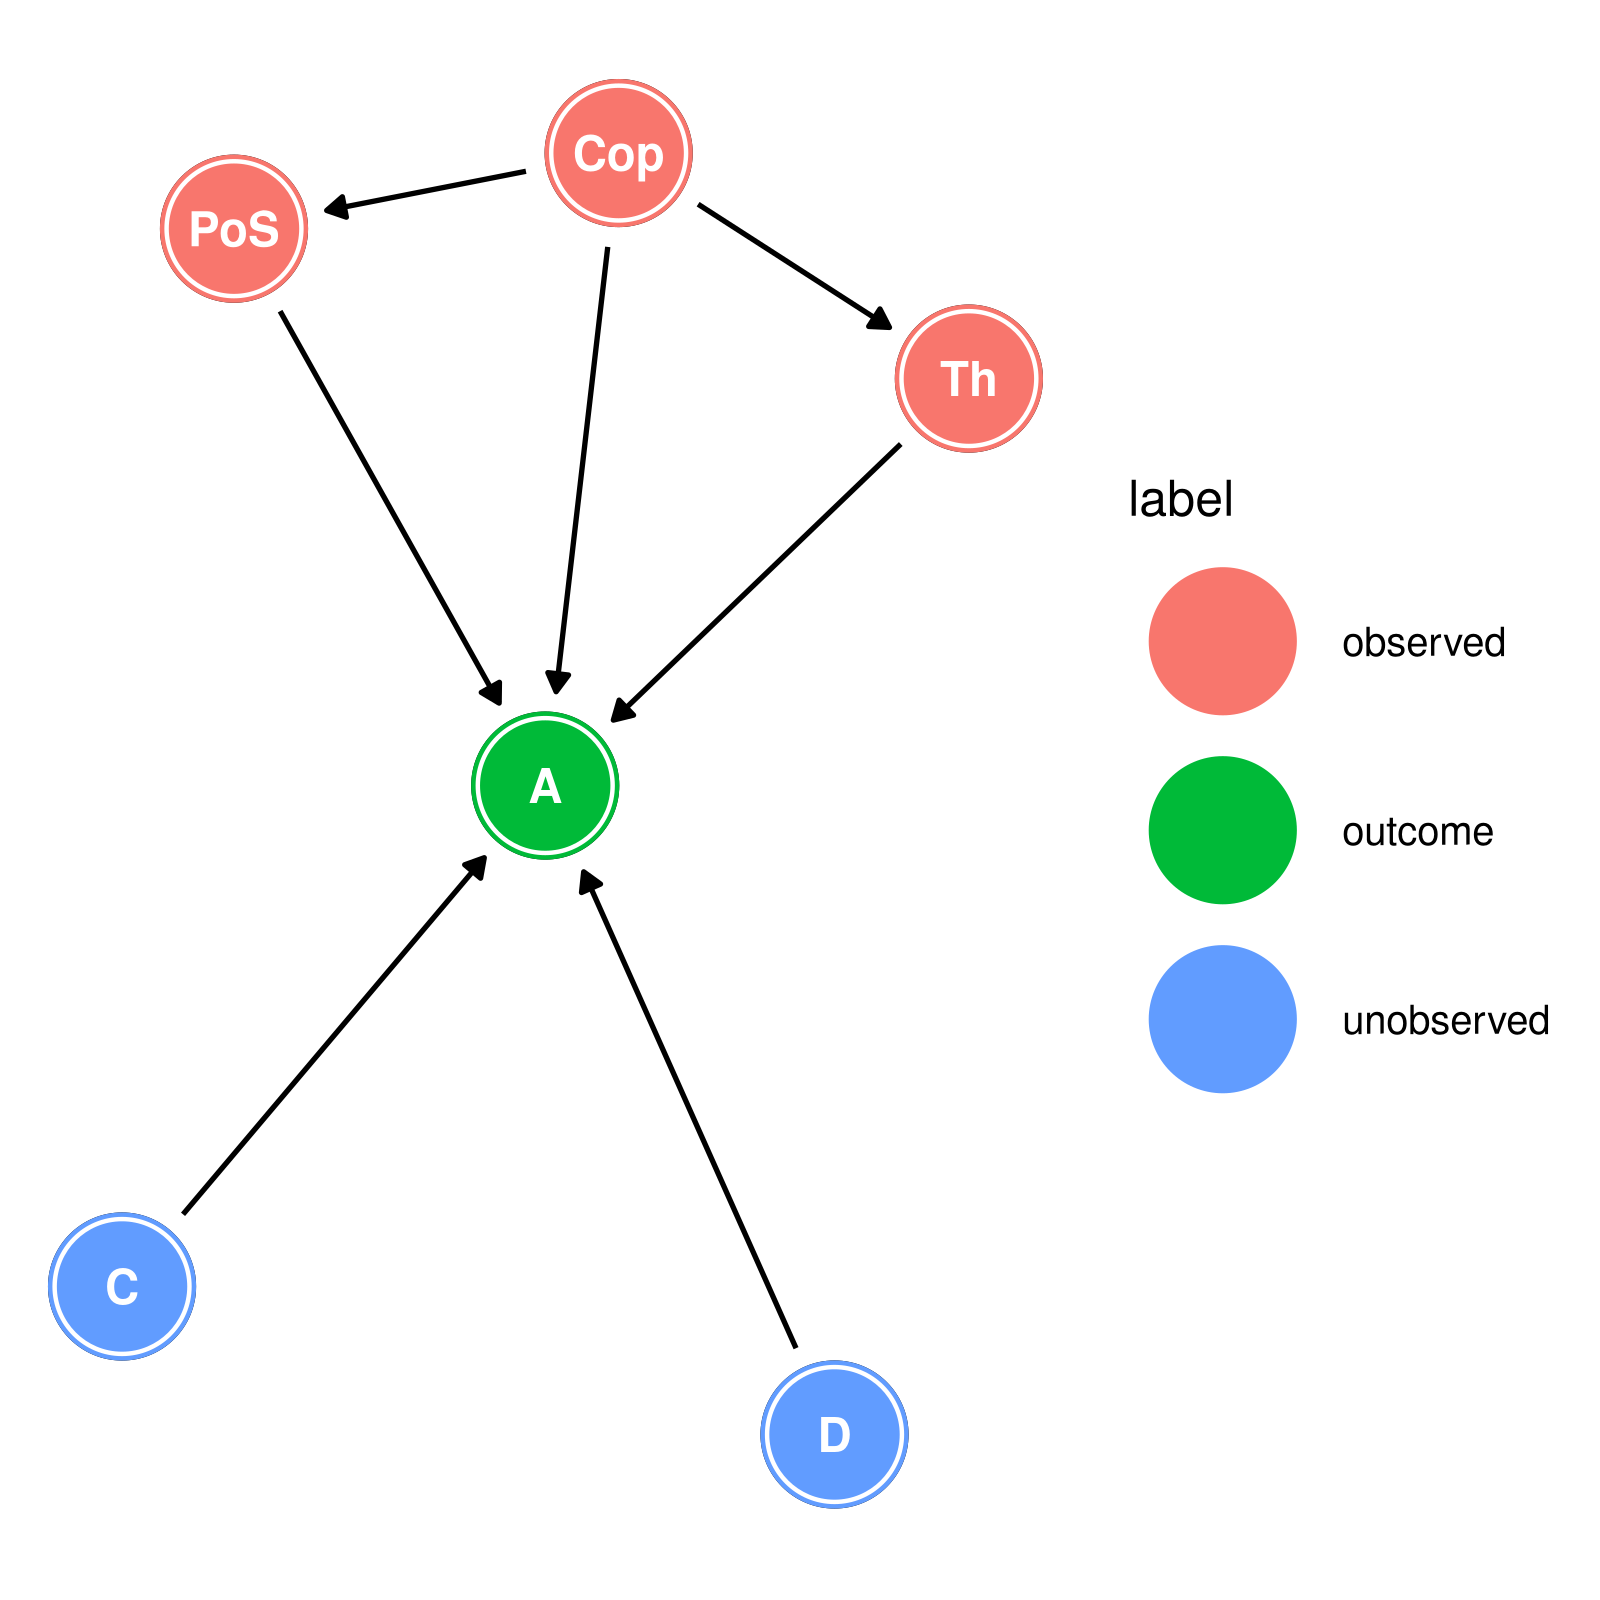
\includegraphics[width=0.65\linewidth]{../analysis/figs/dag_b.png}
	\end{center}
\end{frame}

\begin{frame}
	\frametitle{Issues of dialect and authorship: DAG}
	\begin{center}
	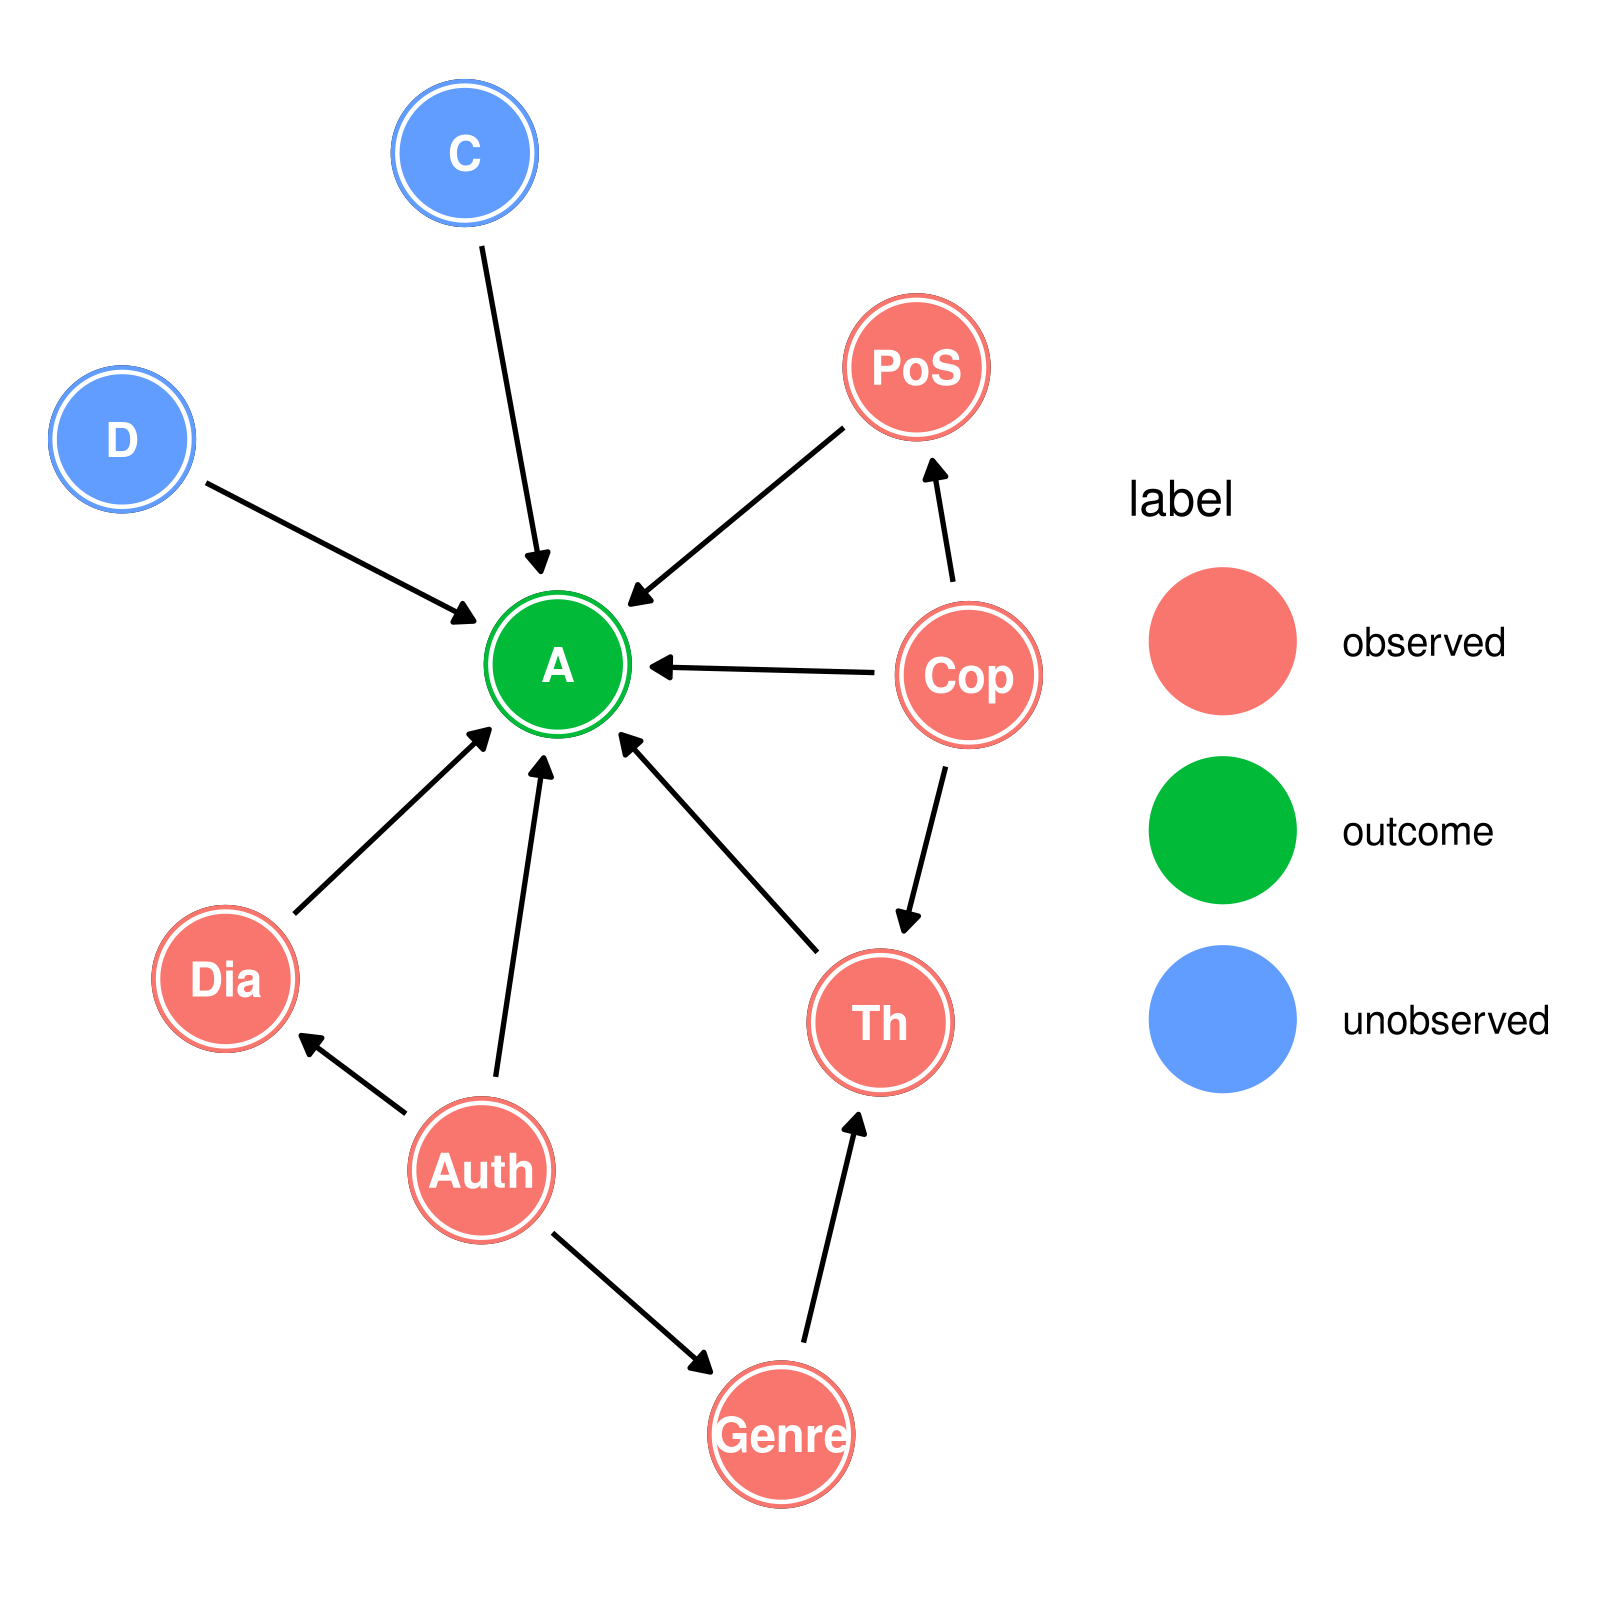
\includegraphics[width=0.65\linewidth]{../analysis/figs/dag_c.png}
	\end{center}
\end{frame}

\begin{frame}
	\frametitle{The target of attraction: distance and precedence}
	\ex.ὡς \textbf{ἀγαθοῖς} τε \textbf{ὑμῖν} προσήκει εἶναι.\\
	That you may be good people. (Xen.\ \emph{Anab.} 3.2.11)

\end{frame}

\begin{frame}
	\frametitle{The target of attraction: final DAG}

	\begin{center}
	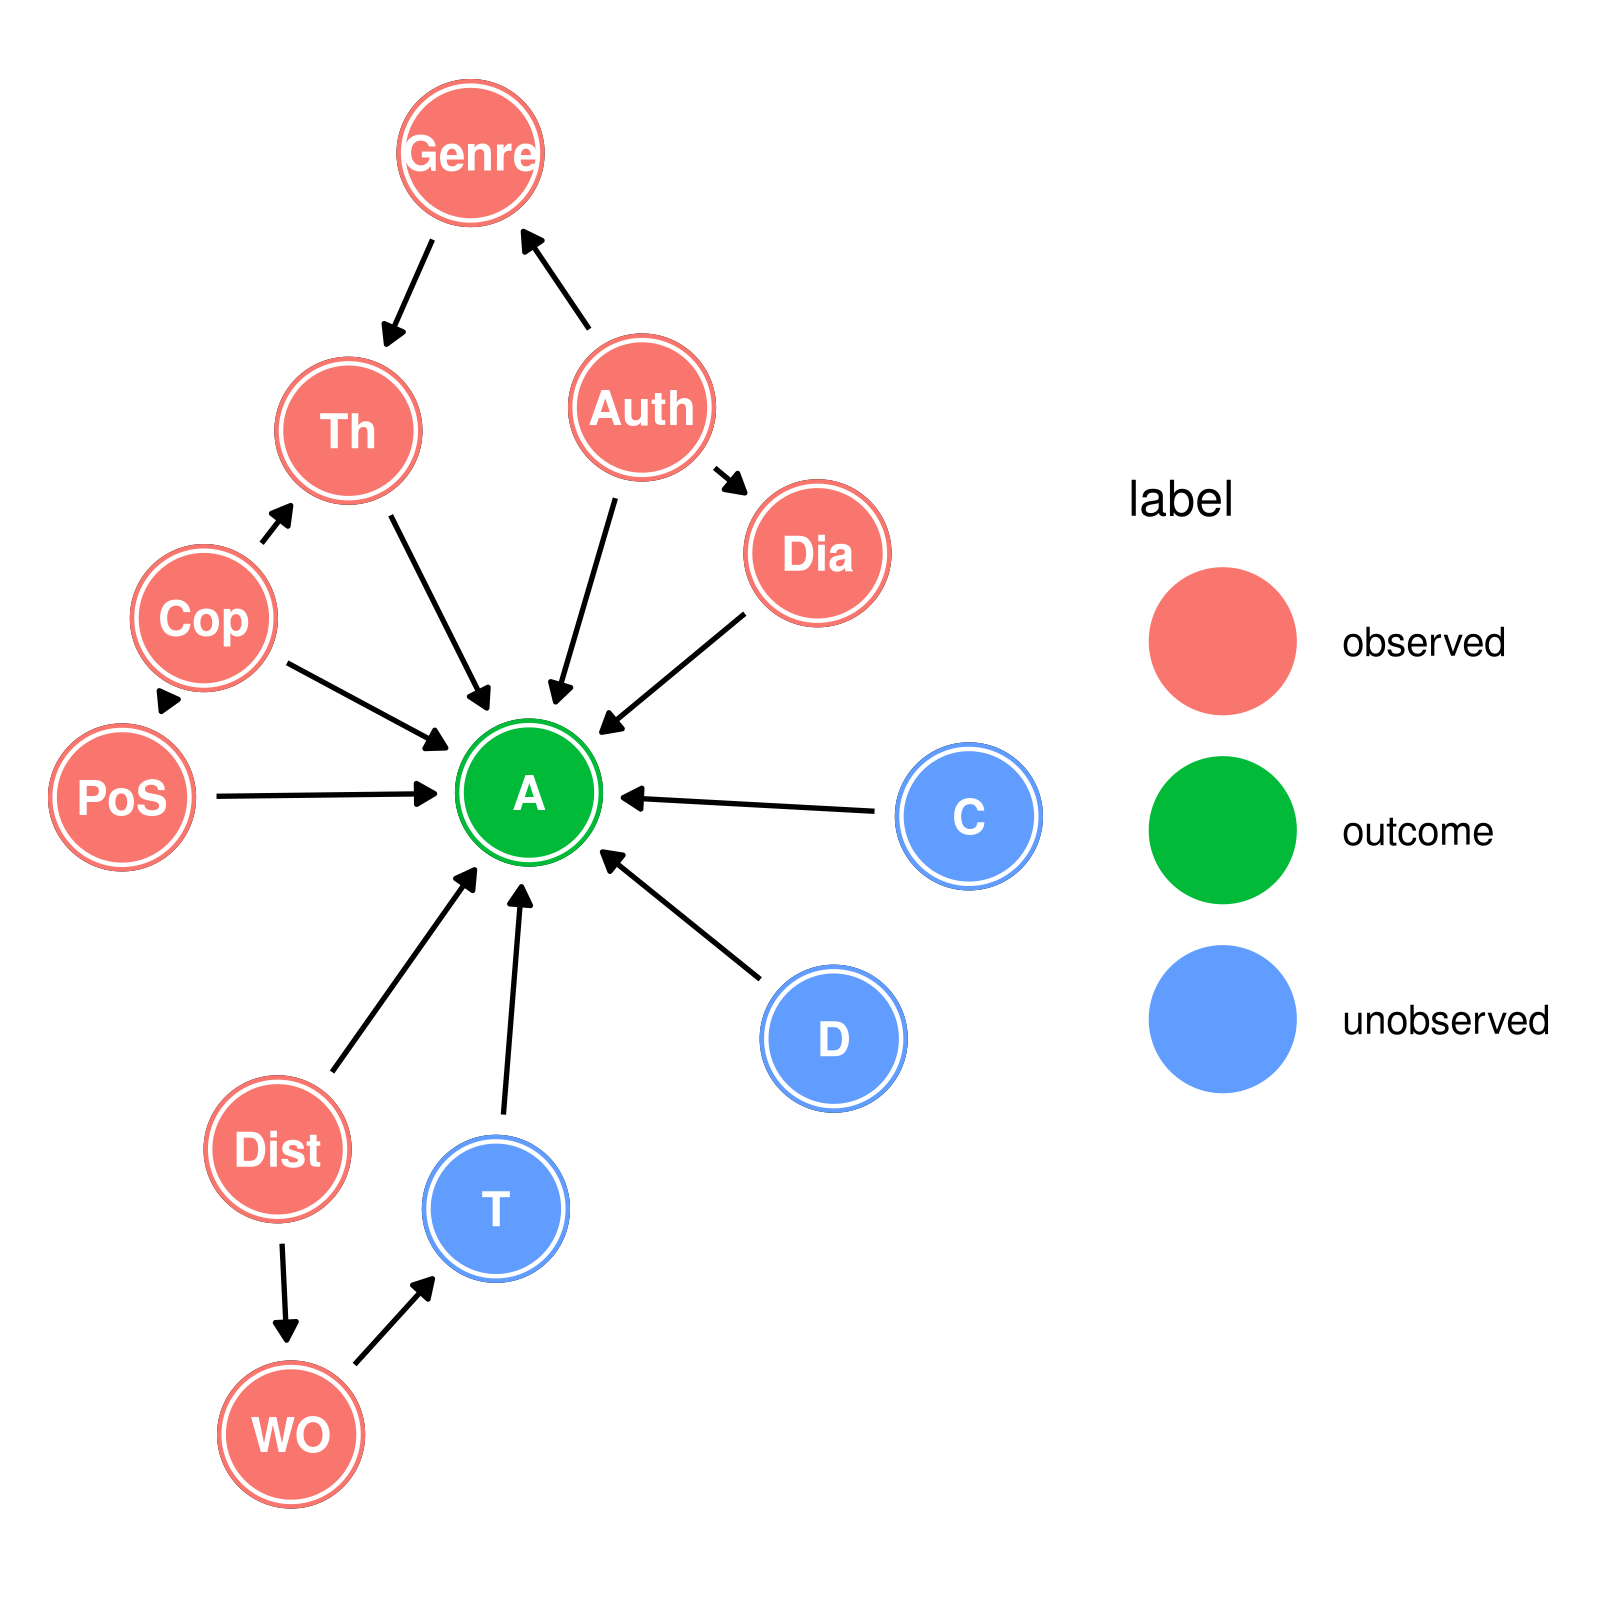
\includegraphics[width=0.60\linewidth]{../analysis/figs/dag_d.png}
	\end{center}

	\vfill


	\footnotesize

	\paragraph{Tooling:} R (\cite{R}), the packages
	\texttt{tidyverse} (\cite{tidyverse}), \texttt{dagitty} (\cite{dagitty}),
	\texttt{ggdag} (\cite{ggdag}), and \texttt{rethinking} (\cite{McElreath2020}),
	as well as the software Stan~(\cite{StanReferenceManual,StanUserGuide}).

\end{frame}

\begin{frame}
	\frametitle{Generalized linear model}
	\small
	\begin{align*}
		\text{A} &\sim \text{Bernoulli}(p_i)\\
		\text{logit}(p_i) &= \alpha + 
		\beta_{\text{Cop}}\text{Cop}_i + 
		\beta_{\text{Dist}}\text{Dist}_i + \beta_{\text{WO}} \text{Prec}_i \\&+
		\beta_{\text{PoS}}\sum^{PoS_{i}-1}_{j=0}{\delta_{j_{\text{PoS}}}} + \beta_{\text{Th}}\sum^{Th_{i}-1}_{j=0}{\delta_{j_{\text{Th}}}} \\&+
			\beta_{\text{Auth}_{i}} + \beta_{\text{Dia}_i}\\
		\alpha &\sim \text{Normal}(0, 1)\\
		\beta_{\text{Cop}}, \beta_{\text{Dist}}, \beta_{\text{Prec}} &\sim \text{Normal}(0, 1)\\
		\beta_{\text{PoS}}, \beta_{\text{Th}} &\sim \text{LogNormal}(0, 1)\\
		\delta_{\text{PoS}}, \delta_{\text{Th}} &\sim \text{Dirichlet}(2)\\
		\beta_{\text{Auth}} &= z_{\text{Auth}}*\sigma_{\text{Auth}}\\
		\beta_{\text{Dia}} &= \overline{\beta}_\text{Dia} + z_{\text{Dia}}*\sigma_{\text{Dia}}\\
		\overline{\beta}_\text{Dia}, z_{\text{Auth}}, z_{\text{Dia}} &\sim \text{Normal}(0,1)\\
		\sigma_{\text{Auth}}, \sigma_{\text{Dia}} &\sim \text{Exponential}(1)
	\end{align*}
\end{frame}

\begin{frame}
	\frametitle{A word on Ordered Categorical Predictors}

	\begin{center}
	\begin{tabular}[t]{ll}
	\toprule
	PoS & Cummulative effect\\
	\midrule
	Participle & $\beta_{\text{PoS}} * 0$\\
	Adjective & $\beta_{\text{PoS}} * (\delta_{\text{Adj}})$\\
	Noun & $\beta_{\text{PoS}} * (\delta_{\text{Adj}} + \delta_{\text{Noun}})$\\
	\bottomrule
	\end{tabular}
	\end{center}

\end{frame}

\begin{frame}
	\frametitle{Copula and Distance}
	\begin{center}
	
\begin{tabular}[t]{lrrrrr}
\toprule
Effect & mean & sd & 5.5\% & 94.5\% & rhat\\
\midrule
$\beta_{\text{Copula}}$ & 2.03 & 0.39 & 1.42 & 2.66 & 1\\
$\beta_{\text{Dist}}$ & -0.22 & 0.04 & -0.29 & -0.16 & 1\\
\bottomrule
\end{tabular}

	\begin{figure}[!h]
	\centering
	\begin{minipage}{.40\textwidth}
		\centering
		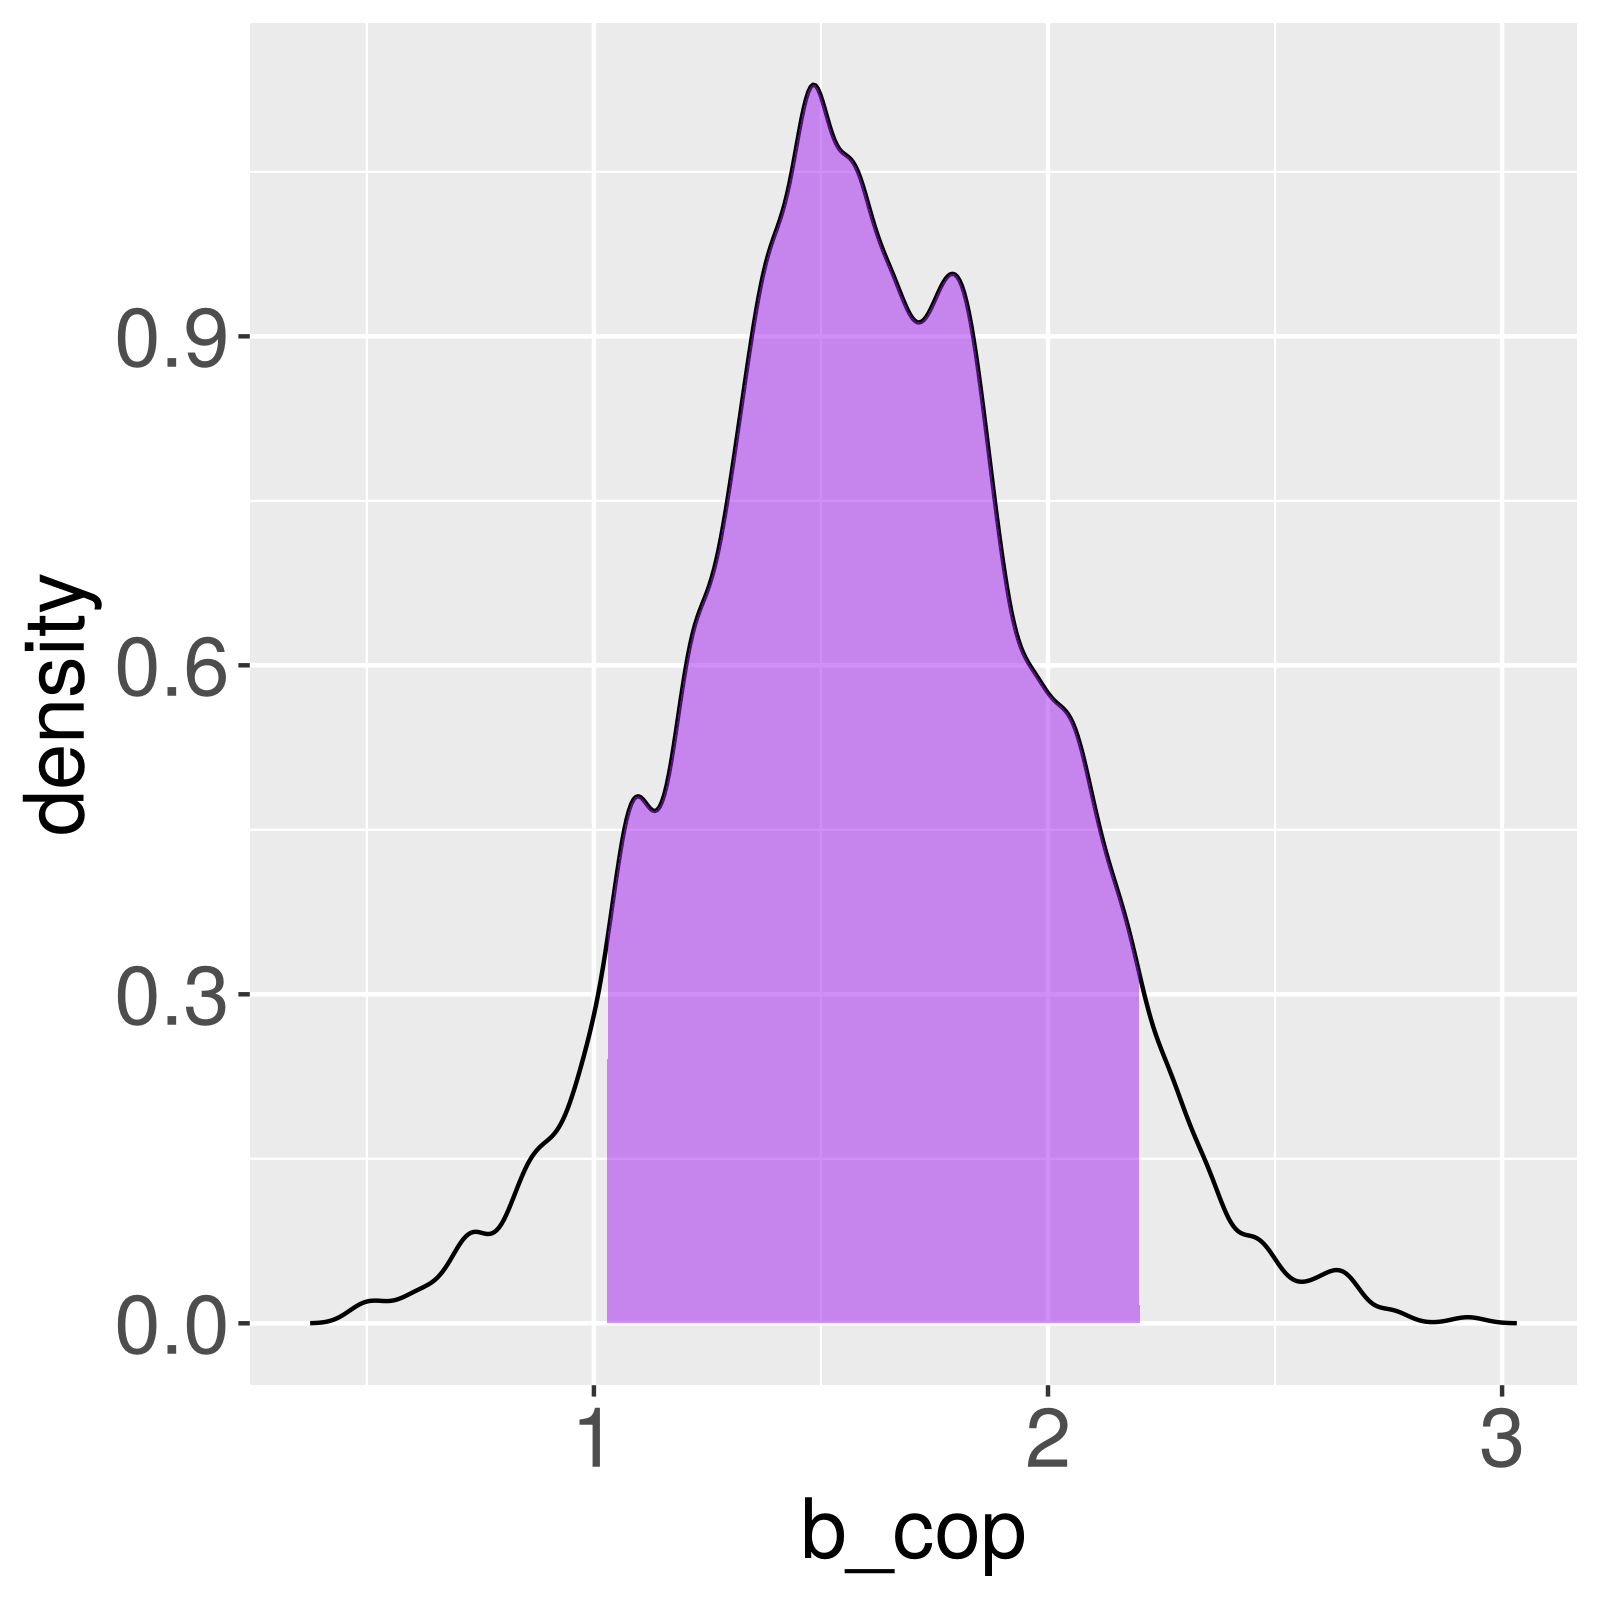
\includegraphics[width=\linewidth]{../analysis/figs/posterior_b_copula.png}
	\end{minipage}%
	\hspace{3em}
	\begin{minipage}{.40\textwidth}
		\centering
		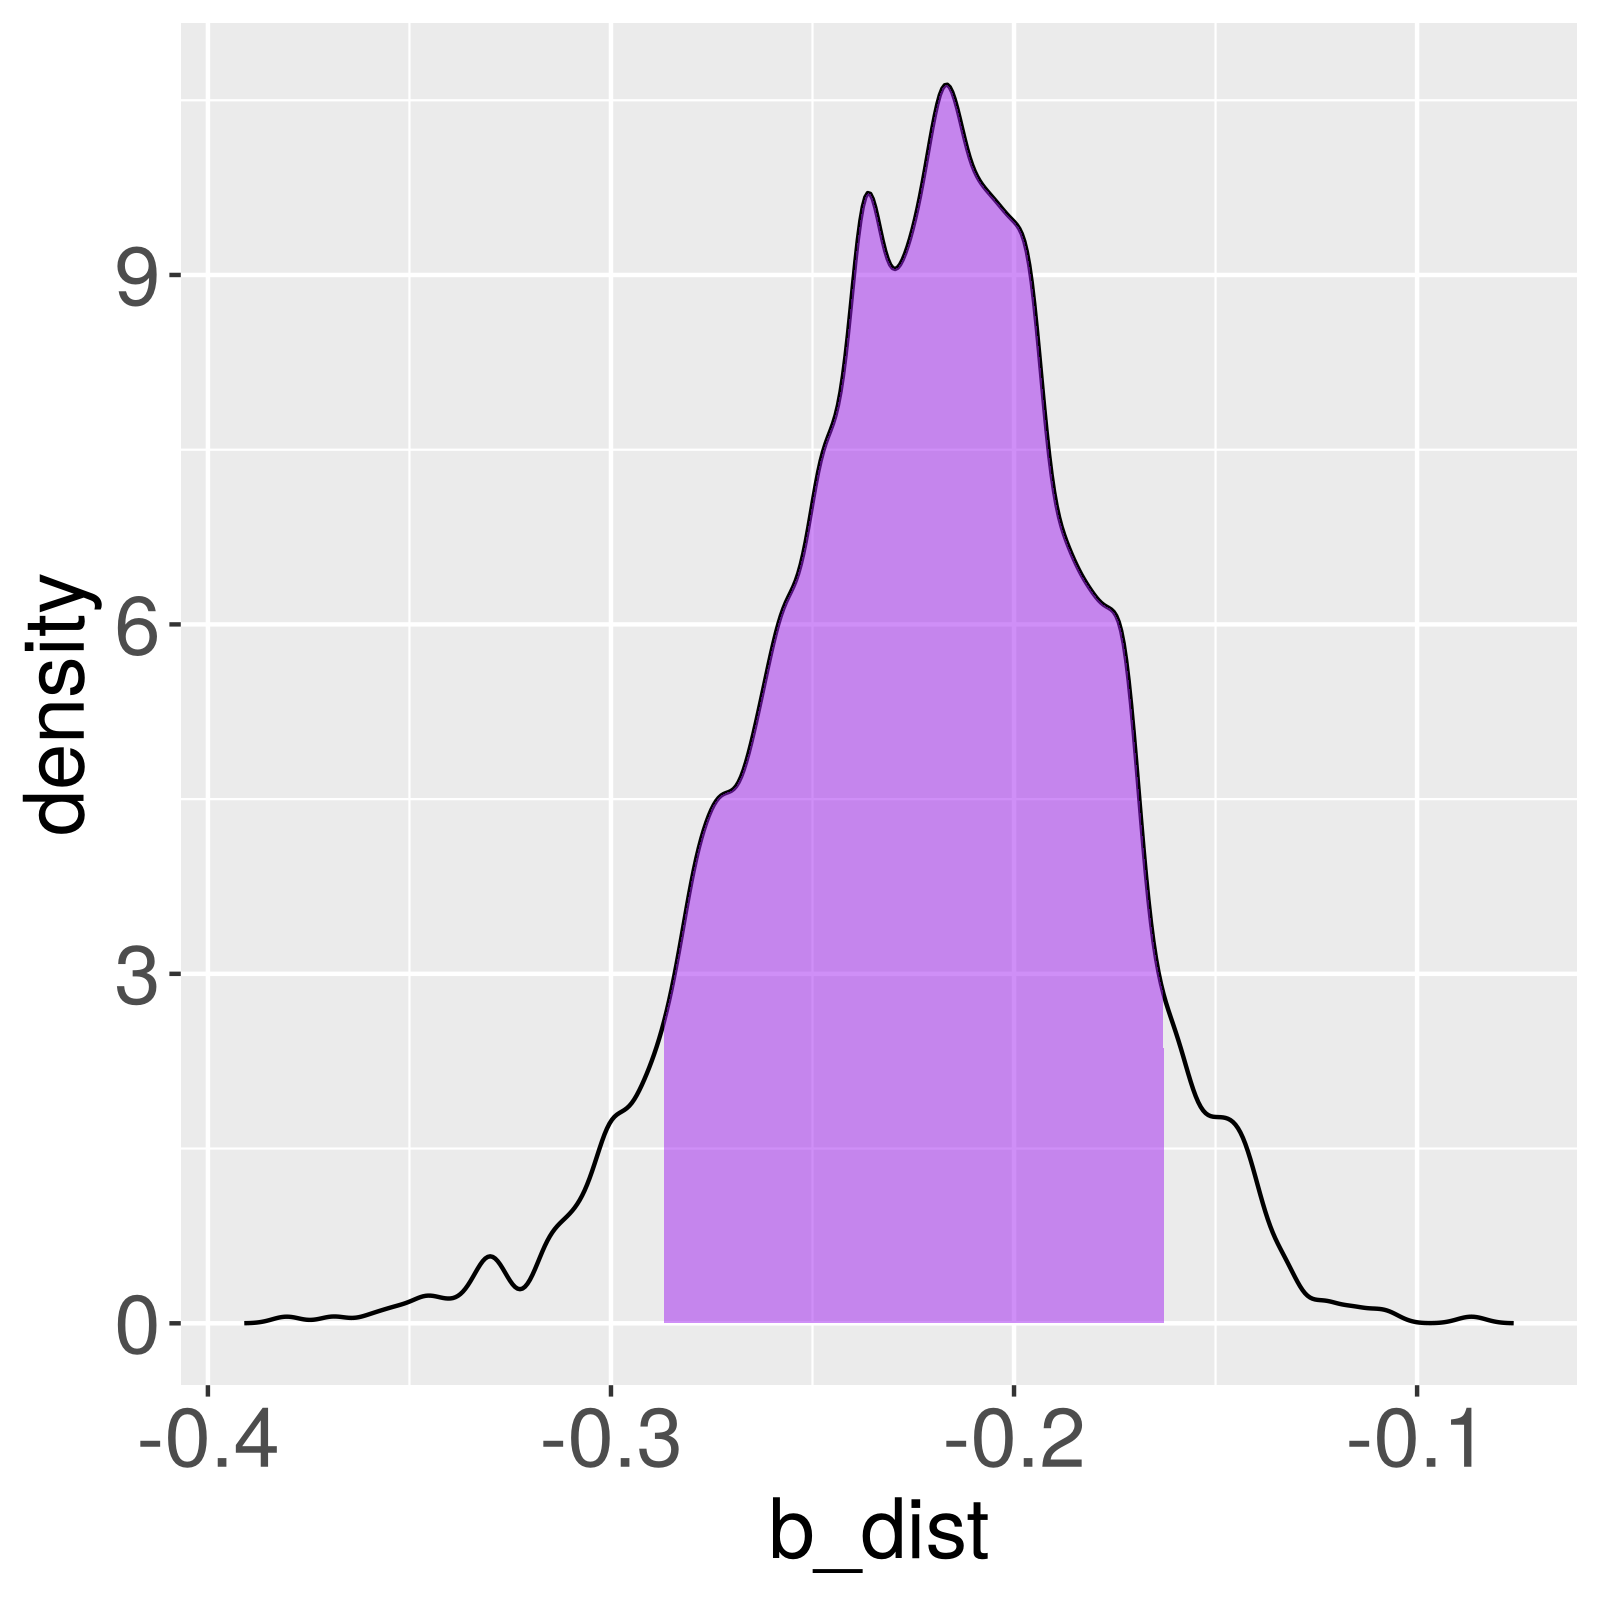
\includegraphics[width=\linewidth]{../analysis/figs/posterior_b_dist.png}
	\end{minipage}
	\end{figure}
	\end{center}

\end{frame}

\begin{frame}
	\frametitle{Part of Speech and the Predicate Hierarchy}
	\small
	\begin{center}
		
\begin{tabular}[t]{lrrrrr}
\toprule
Effect & mean & sd & 5.5\% & 94.5\% & rhat\\
\midrule
$\beta_{\text{PoS}}$ & 0.45 & 0.28 & 0.11 & 0.95 & 1\\
$\delta_{\text{Adj}}$ & 0.53 & 0.18 & 0.23 & 0.82 & 1\\
$\delta_{\text{Noun}}$ & 0.47 & 0.18 & 0.18 & 0.77 & 1\\
\bottomrule
\end{tabular}

		
\begin{tabular}[t]{llrrrrr}
\toprule
PoS & Cummulative effect & mean & sd & 5.5\% & 94.5\% & rhat\\
\midrule
Participle & $\beta_{\text{PoS}} * 0$ & 0.00 & 0.00 & 0.00 & 0.00 & NA\\
Adjective & $\beta_{\text{PoS}} * \delta_{\text{Adj}}$ & 0.25 & 0.18 & 0.05 & 0.60 & 1\\
Noun & $\beta_{\text{PoS}} * (\delta_{\text{Adj}} + \delta_{\text{Noun}})$ & 0.45 & 0.28 & 0.11 & 0.95 & 1\\
\bottomrule
\end{tabular}

	\end{center}
\end{frame}

\begin{frame}
	\frametitle{Thematic Role of the Controller}
	\small
	\begin{center}
		
\begin{tabular}[t]{lrrrrr}
\toprule
Effect & mean & sd & 5.5\% & 94.5\% & rhat\\
\midrule
$\beta_{\text{Theta}}$ & 2.47 & 0.40 & 1.84 & 3.12 & 1\\
$\delta_{\text{Exp}}$ & 0.34 & 0.11 & 0.17 & 0.51 & 1\\
$\delta_{\text{Agent}}$ & 0.66 & 0.11 & 0.49 & 0.83 & 1\\
\bottomrule
\end{tabular}

		\bigskip
		
\begin{tabular}[t]{llrrrrr}
\toprule
Theta & Cummulative effect & mean & sd & 5.5\% & 94.5\% & rhat\\
\midrule
Recipient & $\beta_{\text{Rec}}$ & 1.63 & 0.29 & 1.17 & 2.10 & 1\\
Experiencer & $\beta_{\text{Rec}} + \delta_{\text{Exp}}$ & 1.91 & 0.32 & 1.40 & 2.44 & 1\\
Agent & $\beta_{\text{Rec}} + \delta_{\text{Exp}} + \delta_{\text{Agent}}$ & 2.63 & 0.29 & 2.17 & 3.10 & 1\\
\bottomrule
\end{tabular}

	\end{center}
\end{frame}

\begin{frame}
	\frametitle{Dialect}
	\begin{center}
	\small
\begin{tabular}[t]{lrrrr}
\toprule
Effect & mean & sd & 5.5\% & 94.5\%\\
\midrule
$\overline{\beta}_{\text{Dia}}$ & -0.49 & 0.84 & -1.78 & 0.90 \\
$\sigma_{\text{Dia}}$ & 1.20 & 0.78 & 0.30 & 2.67 \\
$\beta_{\text{Attic}}$ & -0.16 & 0.89 & -1.55 & 1.28 \\
$\beta_{\text{Jonic}}$ & -1.59 & 1.01 & -3.19 & -0.02 \\
$\beta_{\text{Attic}} - \beta_{\text{Jonic}}$ & 1.43 & 0.69 & 0.26 & 2.49 \\
\bottomrule
\end{tabular}
  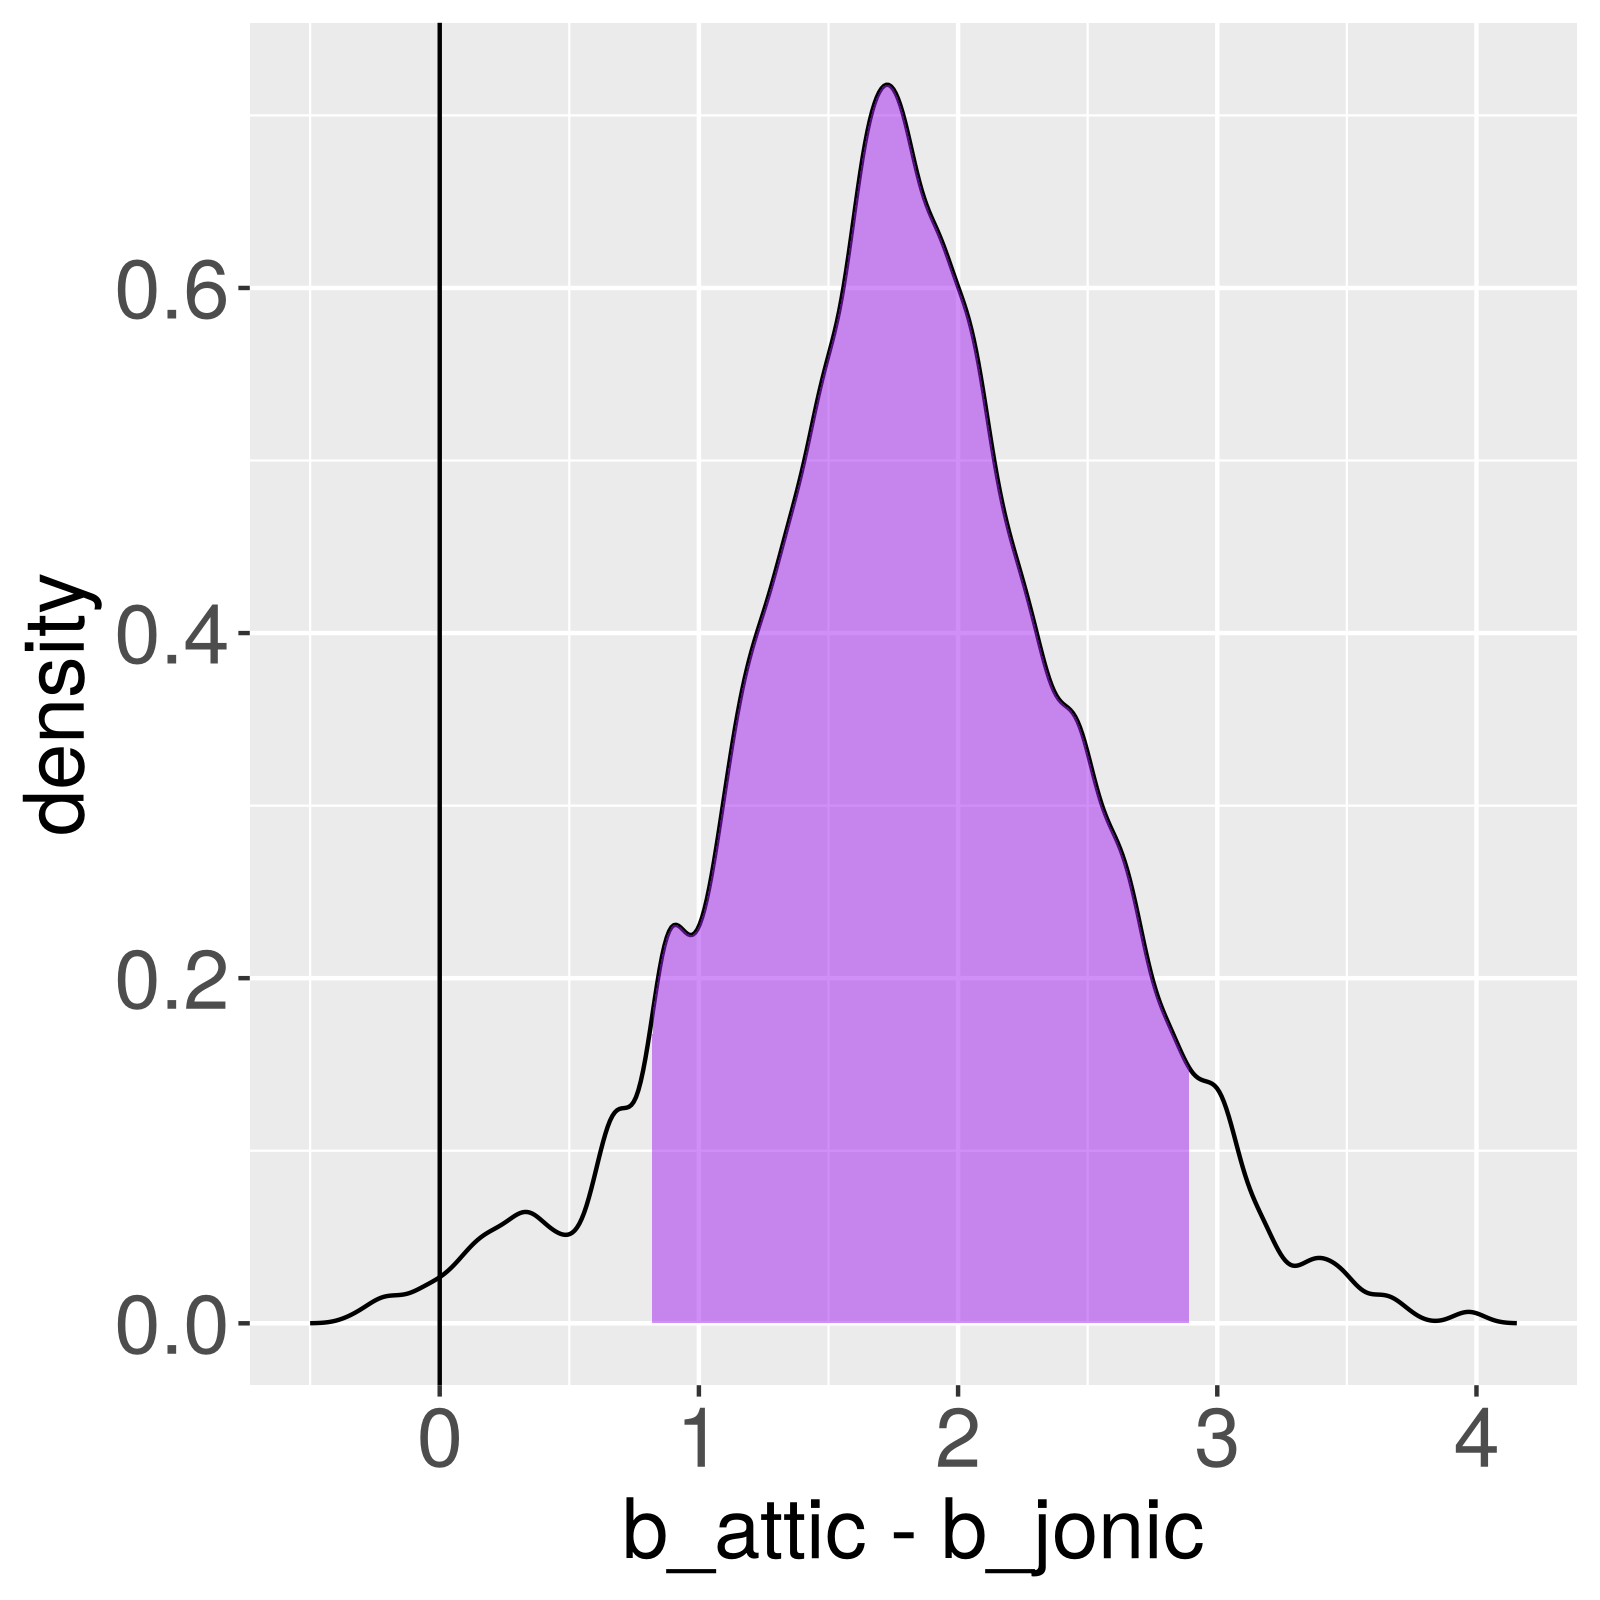
\includegraphics[width=0.4\linewidth]{../analysis/figs/posterior_diff_dia.png}
	\end{center}
\end{frame}

\begin{frame}
	\frametitle{Authorship}
\begin{center}
	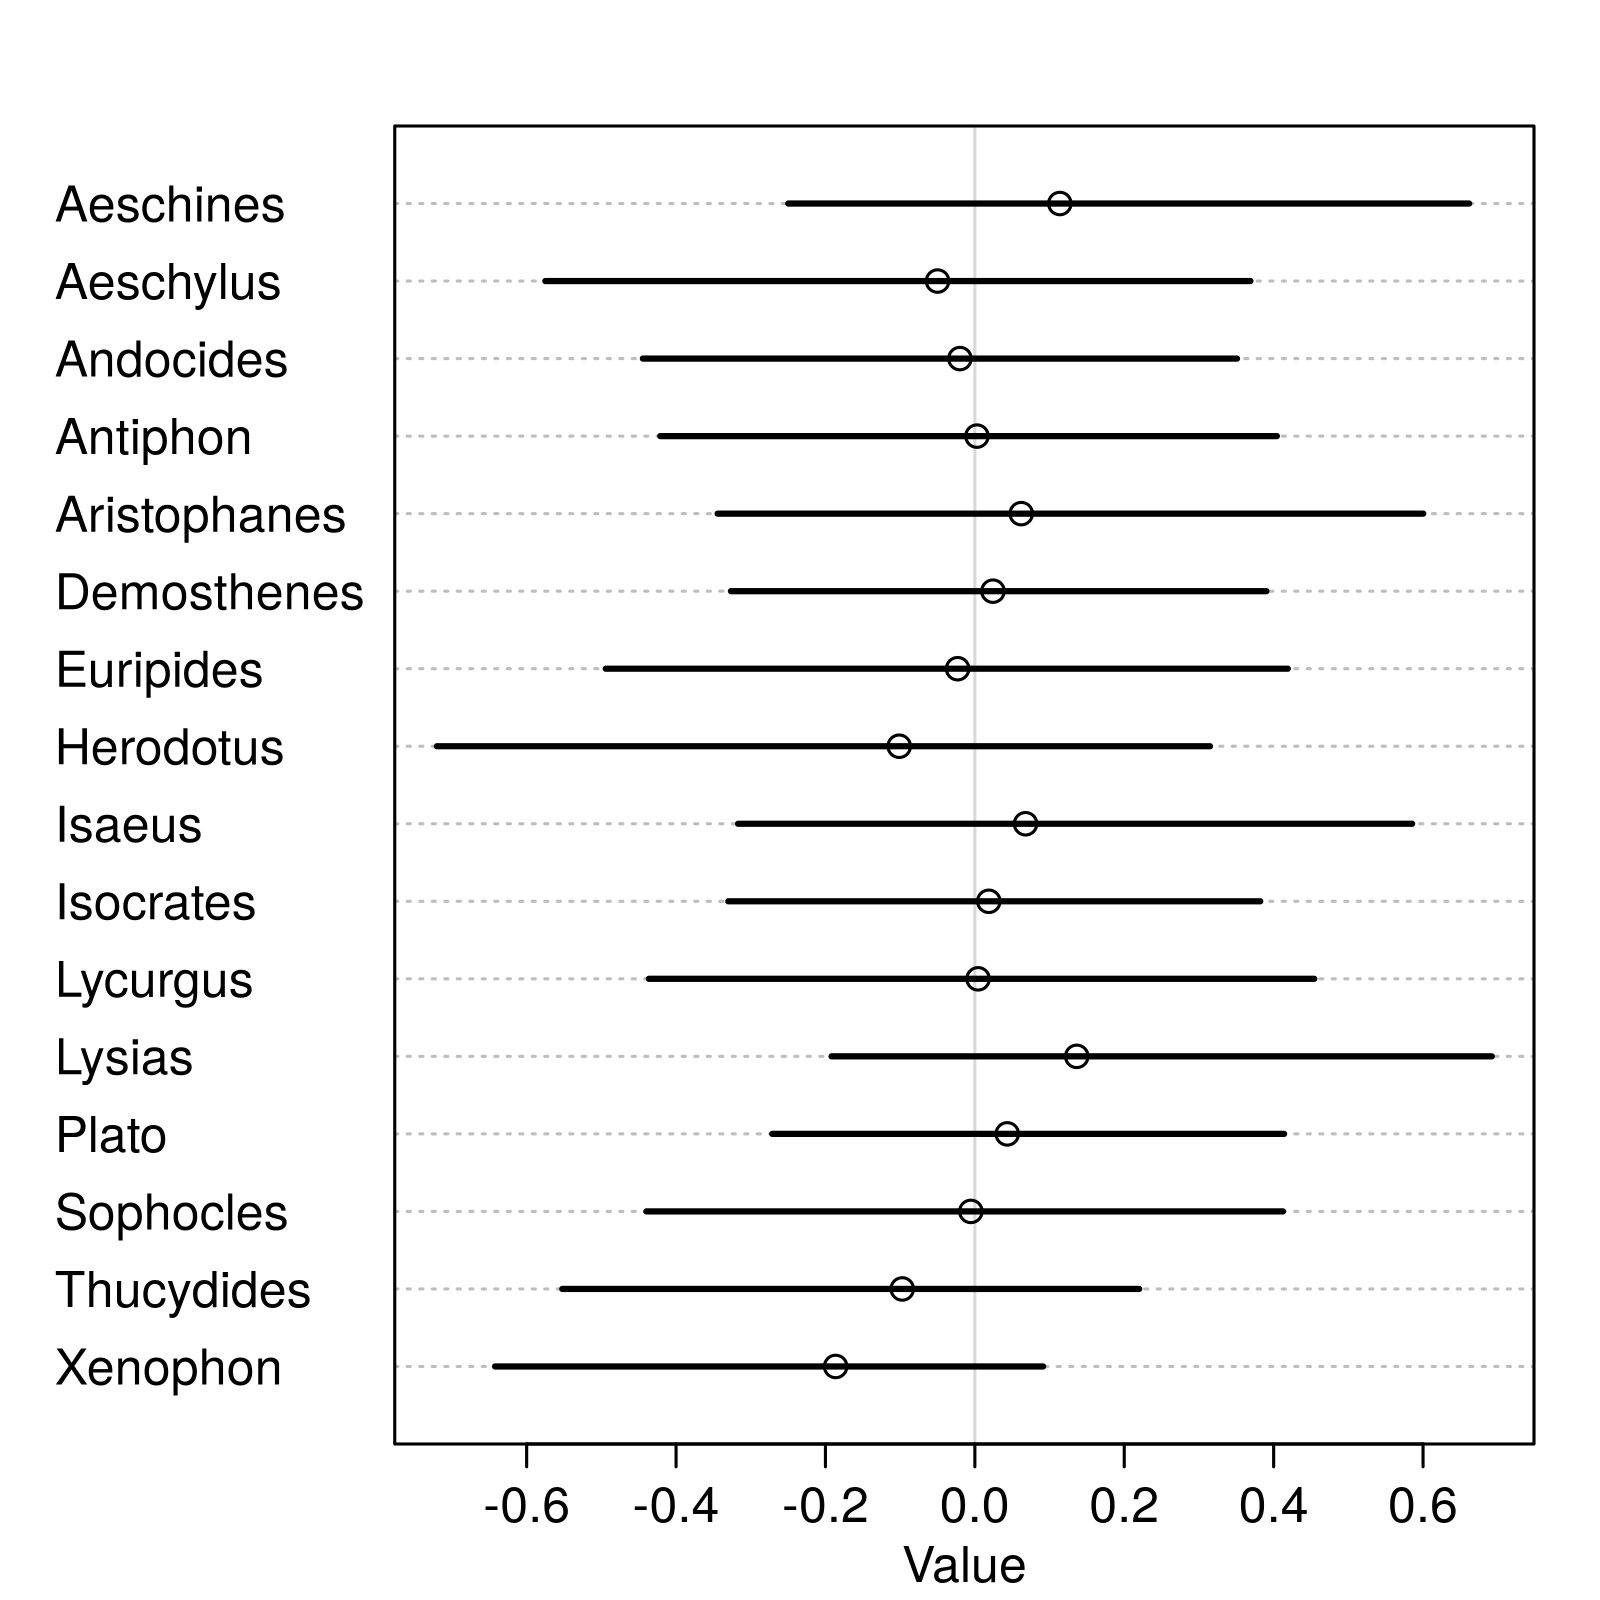
\includegraphics[width=0.70\linewidth]{../analysis/figs/precis_author.png}
\end{center}
\end{frame}

\begin{frame}[standout]
	\large
	Thank you!
	\bigskip

	Contact:\\
	\texttt{caio.geraldes@usp.com}

	Data and code available at\\
	\texttt{github.com/caiogeraldes/icagl2025}
\end{frame}


\end{document}
